\documentclass[a4paper]{article}
\usepackage{graphicx}
%\usepackage{amsmath}
\usepackage[authoryear]{natbib}
%\usepackage{subfig}
% remember to use -sPAPERSIZE=a4 as option to ps2pdf to stop these margins getting corrupted
\usepackage[left=3cm, right=3cm, top=3cm, bottom=3cm, nohead, nofoot]{geometry}
\usepackage{multicol}
\usepackage{nopageno} % removes page numbers
%\usepackage[pdftex]{hyperref} % inserts hyperlinks correctly for PDFs

% Make captions italic
\usepackage[it]{caption}
\renewcommand\captionfont{\itshape}

\usepackage{bar} % bar charts

\bibpunct{[}{]}{,}{n}{,}{,} % citations in format [1], [2,3] etc

% Voodoo for single-column figures and tables - note that they won't float!
\makeatletter
\newenvironment{tablehere}
  {\def\@captype{table}}
  {}
\newenvironment{figurehere}
  {\def\@captype{figure}}
  {}
\makeatother

% Command to put some centred text in a box
\newcommand{\boxit}[1]{
\begin{center}
\noindent \fbox{\parbox{2.7in}{\centerline{#1}}}
\end{center}
}
% Command for scientific notation
\newcommand{\scinot}[2]{ #1\times10^{#2} }

\begin{document}

\title{Building simple, easy-to-use Grids with Styx Grid Services and SSH}

\author{\textbf{Jon Blower$^{*}$}, Keith Haines}
\date{}

\maketitle

\begin{center}
Reading e-Science Centre, Environmental Systems Science Centre, University of Reading, Harry Pitt Building, University of Reading, Whiteknights, Reading RG6 6AL \\
\medskip
$^{*}$ Corresponding author: email address jdb@mail.nerc-essc.ac.uk
\end{center}

\bigskip

\begin{abstract}
Grid systems have a reputation for being difficult to build and use.  We describe how the ease of use of the Styx Grid Services (SGS) software can be combined with the security and trusted nature of the Secure Shell (SSH) to build simple Grid systems that are secure, robust and easy to use and administer.  We present a case study of how this method is applied to a science project (GCEP), allowing the scientists to share resources securely and in a manner that does not place unnecessary load on system administrators.  Applications on the Grid can be run exactly as if they were local programs from the point of view of the scientists.  The resources in the GCEP Grid are diverse, including dedicated clusters, Condor pools and data archives but the system we present here provides a uniform interface to all these resources.  The same methods can be used to access Globus resources via GSISSH if required.
\end{abstract}

\bigskip

\begin{multicols}{2}

\section{Introduction}
As Grid technology matures, an increasing amount of attention is being devoted to the problem of enhancing the usability of Grid systems.  It is a well-known problem~\cite{chin:2004} that many Grid toolkits (e.g.\ Globus~\cite{globustoolkit}) are difficult to install and use on both the client and server side.  Futhermore, these toolkits often require a large number of incoming ports to be open on the server (and the client), which is sometimes inconsistent with local security policy.

Grid computing is usually defined as distributed computing performed transparently across multiple administrative domains.  This definition does not mandate the use of complex Grid middleware.  We believe that perfectly functional Grids can be created using simple, well-understood software in a manner that is friendly to both users and resource providers.

\subsection{The problem of usability}
Despite many advances in Grid usability, there is still much scope for further increasing the ease of use of Grid technology.  Users typically have to perform multiple steps of resource selection, file transfer, job submission and job monitoring in order to run even simple Grid jobs.  The aim of the Styx Grid Services system~\cite{blower:2006} is to make it as easy as possible for novice users to use Grid systems by {\em making the running of applications on a Grid as easy as running applications on the user's own computer\/}.  In this paper we shall describe how the Styx Grid Services system can be adapted for use in more secure environments, whilst retaining its essential quality of being easy to install and use.

\subsection{The problem of security}
A key problem in the design of Grid systems is security.  It is very important to find a level of security with which both users and resource providers can be satisfied.  If the security level is too low there will be an unacceptable risk that the resource in question will be compromised by unauthorized access.  Conversely, if the security level is too high, many users will find it too difficult to use the resource; in this case, users will either choose not to use the resource in question or, worse, users will find ways to circumvent the security mechanism.

A good example of this is the Grid Security Infrastructure (GSI~\cite{gsi}), which is based on public-key infrastructure and proxy certificates.  This security mechanism gives, theoretically, a high level of security; however, it often raises complaints from users who feel that this level of security interferes with their normal working practices to an unacceptable degree.  Many users feel that the processes of caring for their digital certificates, renewing them annually and generating time-limited proxies before running jobs are too cumbersome.  This user-unfriendliness leads some users to engage in forbidden practices such as storing their digital certificates in multiple, perhaps insecure, locations and sharing their digital certificates with colleagues~\cite{beckles:2005}.  The resource administrator has no control over these practices and cannot detect that they are occurring.

Some Grid systems (e.g.\ the NERC Data Grid) take the approach of completely insulating the user from the certificate-based security architecture by storing users' certificates in some secure location such as a MyProxy server and allowing the users to log on to the Grid using a username and password.  Whenever the certificate is needed, it is automatically retrieved in a manner that is hidden from the user.  This ``portal'' approach is one of the best means for increasing the usability of Grid security but does require a system administrator to care for the certificates on behalf of the users.

\subsection{Why not use SSH and SFTP?}
At heart, many Grid jobs consist of transferring input files to a Grid resource, running the job and transferring the output files back to the user.  A common question that is asked by users is, ``Why can't I simply use the Secure Shell (SSH) and Secure FTP (SFTP, or its legacy equivalent SCP) to run my jobs?''  SSH and SFTP are 
well-known utilities with which a large proportion of users are already familiar.  Files can be transferred to and from remote resources securely with SFTP.  Applications can be run on remote machines through SSH.  Importantly, SSH and SFTP are very familiar to system administrators (sysadmins).  Sometimes, sysadmins will {\em only\/} permit remote access to their resources through SSH.

In order to log on to a remote resource using SSH, the user must have an account on that resource.  Therefore, if the user wishes to access many resources, he or she will need an account on each of those resources.  At first glance, this would seem to violate the principle of ``single sign-on'', in which the user can access multiple resources having authenticated only once.  Single sign-on is one of the problems that GSI addresses through the use of user certificates.  However, in practice many systems that use GSI also require that each user has a unique user account on each resource: the user's certificate is then simply mapped to this account.  Single sign-on can be achieved in the SSH domain through the use of public and private keys and authentication agents.  Computer-savvy users who dislike the GSI method of authentication have been known to take unusual steps in order to obtain a plain SSH connection (e.g.\ running an SSH server as a Grid job and then logging into it).

For many Grids, particularly those with a relatively small number of users and for which little administrative effort is available, we believe that the use of SSH in place of more complex systems is perfectly acceptable.  A well-administered SSH-based system is likely to be {\em more\/} secure than a more complex system that is not properly administered, and in which users engage in poor security practices.

\subsection{The proposed solution}
In this paper we shall describe how the ease of use of the Styx Grid Services system can be combined with the security of SSH to allow Grids to be constructed simply, allowing users to run Grid jobs with very little effort and placing very little load on system administrators.  The combined system is known as SGS-SSH.  For resource providers that must use GSI security, GSISSH can be used in place of SSH with little additional effort; no more middleware (e.g.\ the rest of the Globus Toolkit) is necessary.

We shall illustrate our solution through a case study.  The GCEP (Grid for Coupled Ensemble Prediction) project is a NERC e-Science project that will study the predicability of the Earth's climate on seasonal to decadal timescales.  In GCEP, users will run jobs on a Grid of machines in several different institutions, including the UK National Grid Service (NGS).  Our solution will allow users to run Grid jobs just as easily as if they were running programs on their local machines.  Furthermore, the administrators of the machines in the Grid will not be burdened by the tasks of installing and maintaining complex pieces of software.

Before we describe how the SGS-SSH system is constructed, we shall summarize the key benefits of the Styx Grid Services system for enhancing the ease of use of Grids.

\section{How Styx Grid Services make Grids easy to use}
The Styx Grid Services (SGS) system is a means for running remote applications {\em exactly\/} as if they were installed locally.  The software is pure Java, is very small in size (under 3 MB) and is easy to install and configure.  The technical details of the SGS system have been discussed in previous papers~\cite{blower:2005,blower:2006} and will not be repeated here.  To illustrate how the SGS system is installed and used, we shall work through a concrete example.

Let us take the example of a simple visualization program called {\tt makepic} that reads an input file and creates a visualization of the results as a PNG file.  The names of the input and output files are specified on the command line, for example:

\begin{verbatim}
makepic -i input.dat -o pic.png
\end{verbatim}

This program can be deployed on a server as a Styx Grid Service as follows.  The {\tt makepic} program is installed on the server.  A simple XML configuration file is created on the server.  This file describes the program in terms of its inputs, outputs and command-line arguments (see figure~\ref{fig:makepicconfig}).  The SGS server daemon is then started.

\begin{figure*}
\centering
\begin{verbatim}
<gridservice name="makepic" command="/path/to/makepic">
  <params>
    <param name="inputfile" paramType="flaggedOption" flag="i" required="yes"/>
    <param name="outputfile" paramType="flaggedOption" flag="o" required="yes"/>
  </params>
  <inputs>
    <input type="fileFromParam" name="inputfile"/>
  </inputs>
  <outputs>
    <output type="fileFromParam" name="outputfile"/>
    <output type="stream" name="stdout"/>
  </outputs>
</gridservice>
\end{verbatim}
\caption{Portion of the configuration file on a Styx Grid Services server, describing the {\tt makepic} program that is deployed.  This specifies that the program expects one input file, whose name is given by the command-line argument following the ``-i'' flag.  The program outputs one file, whose name is given by the command-line argument following the ``-o'' flag, and also outputs data on its standard output stream.}
\label{fig:makepicconfig}
\end{figure*}

Clients can now run the {\tt makepic} Styx Grid Service from remote locations, exactly as if the {\tt makepic} program were deployed on their local machines.  They do this using the {\tt SGSRun} program, which is a generic client program for running any Styx Grid Service:

\begin{verbatim}
SGSRun <hostname> <port>  \
   makepic -i input.dat -o pic.png
\end{verbatim}
where {\tt <hostname>} and {\tt <port>} are the host name (or IP address) and port of the SGS server respectively.  The {\tt SGSRun} program connects to the SGS server and downloads the XML description of the {\tt makepic} program  (figure~\ref{fig:makepicconfig}).  {\tt SGSRun} uses this configuration information to parse the command line arguments that the user has provided.  It then knows that {\tt input.dat} is an input file and uploads it automatically from the user's machine to the SGS server before the program is started.  Having started the program, {\tt SGSRun} knows that {\tt makepic} will produce an output file called {\tt pic.png}, which it downloads to the user's machine.

It is a very easy task to create a simple shell script (or batch file in Windows) called {\tt makepic} that wraps the {\tt SGSRun} program and contains the host name and port of the SGS server, so the user can simple run:

\begin{verbatim}
makepic -i input.dat -o pic.png
\end{verbatim}
exactly as before.  Many scientific codes have corresponding graphical wrapper programs that use the command-line executable as an ``engine'', display results graphically and perhaps allow the user to interact with the running program.  The {\tt makepic} script (which calls the remote Styx Grid Service) behaves identically to the original executable and so could be called by such a graphical wrapper program, thereby ``Grid-enabling'' the graphical program without changing it at all.  More details on this process can be found on the project website~\cite{sgswebsite}.

By allowing the user to execute programs on a Grid exactly as if they were local programs, the Styx Grid Services software provides a very natural and familiar environment for users to work in.  Users do not have to know the details of where or how the remote program runs, nor do they need to manually upload input files to the correct location: once the program is deployed as a Styx Grid Service, all this is handled automatically.

\subsection{Styx Grid Services and workflows}
Given that, in the SGS system, remote services can be executed exactly as if they were local programs, simple shell scripts can be used to combine several remote services to create a distributed application or ``workflow''.  This is described in detail in~\cite{blower:2006}.  No special workflow tools are required on either the client or server side to do this.  Data can be transferred directly between applications along the shortest network route, saving time and bandwidth (i.e.\ intermediate data do not have to pass through the client).  It should be noted that this method does not provide all the features that might be required of a general workflow system but will be sufficient for many users.

\subsection{Running jobs on Condor and Sun Grid Engine via SGS}\label{sec:condor_sge}
In the above example the {\tt makepic} program runs on the SGS server itself.  By using a distributed resource management (DRM) system such as Condor~\cite{condor} or Sun Grid Engine (SGE,~\cite{sungridengine}), the program can be run on a different machine, balancing the load between a set of machines in a Condor pool or cluster.  With a very small change to the SGS configuration file, the SGS system can run programs through Condor or SGE in a manner that is completely transparent to the user: the client interface is identical in all cases.  Plugins to allow the SGS system to run jobs on other DRMs such as PBS (Portable Batch System) can be created if required.

This is particularly useful when the user wishes to execute the same program many times over a number of input files.  This is known as ``high-throughput computing'' and is commonly used in Monte Carlo simulations and parameter sweep studies.  In the above example, the user might wish to execute the {\tt makepic} program over a large number of input files, creating a visualization of each one.  Normally this would require the user to upload the input files, name them in some structured fashion and create an appropriate job description file in a format that is understood by Condor, SGE or the DRM system in question.

In the Styx Grid Services system, the running of these high-throughput jobs is very simple.  Let us imagine that the user has a set of input files for the {\tt makepic} program in a directory called {\tt inputs} on his or her local machine.  The user simply runs the {\tt makepic} Styx Grid Service as before but, instead of specifying a single input file on the command line, the user enters the name of the {\tt inputs} directory:

\begin{verbatim}
makepic -i inputs -o pic.png
\end{verbatim}
where {\tt makepic} is the script that wraps the {\tt SGSRun} executable as described above.

The input files are automatically uploaded to the SGS server as before.  The server notices the presence of an input directory where it was expecting a single file.  It takes this as a signal to run the {\tt makepic} program over each file in the input directory, producing a picture for each file.  The client then downloads these pictures automatically and places them in a directory called {\tt pic.png} on the user's local machine.  The SGS server uses the underlying DRM system (e.g.\ Condor or SGE) to run these tasks in parallel on the worker nodes.  The progress of the whole job is displayed to the client as the individual tasks are executed.

\subsection{Disadvantages of the SGS system}
The design of the SGS system has focused on ease of use, deployment and maintenance.  There are a number of disadvantages of the system:
\begin{itemize}
\item It only works with command-line programs (this is true for most Grid systems).
\item The current SGS system will not work well in cases where the output files that are produced by a program are not predictable, or where the program spawns other programs during execution.  Work is underway to address this limitation.
\item The SGS system has its own security model.  The server administrator must maintain an SGS user database in addition to that of the underlying system.
\item On the server, each application runs with the permissions of the owner of the SGS server itself, rather than with the permissions of the specific user.
\item Some resource providers might not trust the SGS software without considerable further testing and wider acceptance within the community.
\end{itemize}

\section{SGS-SSH}
The last three issues in the above list can be addressed by combining the SGS system with the Secure Shell (SSH).  Essentially, the user uses the SGS system exactly as before (and benefits from its ease of use) but mutually authenticates with the server using SSH.  All SGS traffic is transmitted over the secure channel that is created by the SSH connection.  This combined system is known as SGS-SSH.

This is achieved through a relatively small modification to the SGS software.  The original SGS server reads and writes messages through network sockets.  The SGS-SSH ``server'' is actually a program that reads messages on its standard input and writes replies to its standard output.  The SGS client is modified to connect to the remote server via SSH and execute the SGS-SSH ``server'' program via an exec request.  The client then exchanges messages with the SGS-SSH server program through the secure channel.

Therefore, the only server that needs to be maintained by the system administrator is the SSH server itself.  The user authenticates via the normal SSH procedures and the applications that the user runs through the SGS-SSH interface run with the permissions of the specific user in question, not a generic user.  There is no separate user database.

One might ask what the value is of using the Styx Grid Services system at all - why not simply use SFTP and SSH?  There are a number of advantages of the SGS system in this environment:

\begin{itemize}
\item The SGS system automatically takes care of uploading the input files and downloading the output files to and from the Grid resource.
\item The SGS system saves the user from having to manually create job submission files for DRM systems such as Condor and SGE (section~\ref{sec:condor_sge} above).
\item The SGS system automatically monitors the progress of jobs and displays this to the user.
\item By running the application through an intermediary program (i.e.\ the SGS server program), there is an opportunity to automatically harvest metadata about each run.  One could keep a record of each invocation of a particular program on the Grid and automatically store metadata about each run (this metadata could be provided by the user from the {\tt SGSRun} program).
\end{itemize}

\section{Case Study: the GCEP project}
GCEP (Grid for Coupled Ensemble Prediction) is a NERC e-Science project that involves the Reading e-Science Centre (ReSC), the NERC Centre for Global Atmospheric Modelling (CGAM), the British Antarctic Survey (BAS) and the Council for the Central Laboratory of the Research Councils (CCLRC).  GCEP aims to test the extent to which the Earth's climate can be predicted on seasonal to decadal timescales.  This will be achieved by running a large number of computer-based climate simulations, with each simulation being started from a different set of initial conditions of the oceans and the distributions of ice, soil moisture and snow cover.  If any aspect of climate can be predicted on these timescales, it is these slowly-varying properties that will contain the necessary information.

The climate simulation program that will be run is the Hadley Centre's full HadCM3 model~\cite{hadcm3}, which has recently been ported so that it can run on PC clusters.  Large numbers ({\em ensembles\/}) of simulations will need to be run in order to gather the necessary statistics.  The process of analysing the results of the simulations will also be compute- and data-intensive.  The compute resources available to the project include clusters at ReSC, BAS and CCLRC, a Condor pool at the University of Reading and the UK National Grid Service (NGS).  The project will generate several terabytes of data and so an efficient data management system will be required to allow results to be shared amongst the project scientists.

\subsection{GCEP Grid architecture}

The GCEP partners wish to focus on the science challenges and do not wish to devote large amounts of time to the installation and maintenance of complex Grid middleware.  We propose to use SGS-SSH to build the Grid.  In this way, the administrators of the GCEP clusters (at ReSC, BAS and CCLRC) only need to maintain an SSH server and set up a local user account for each of the GCEP users.  Figure~\ref{fig:gcep} gives an overview of the proposed GCEP architecture.

\begin{figure*}
\centering
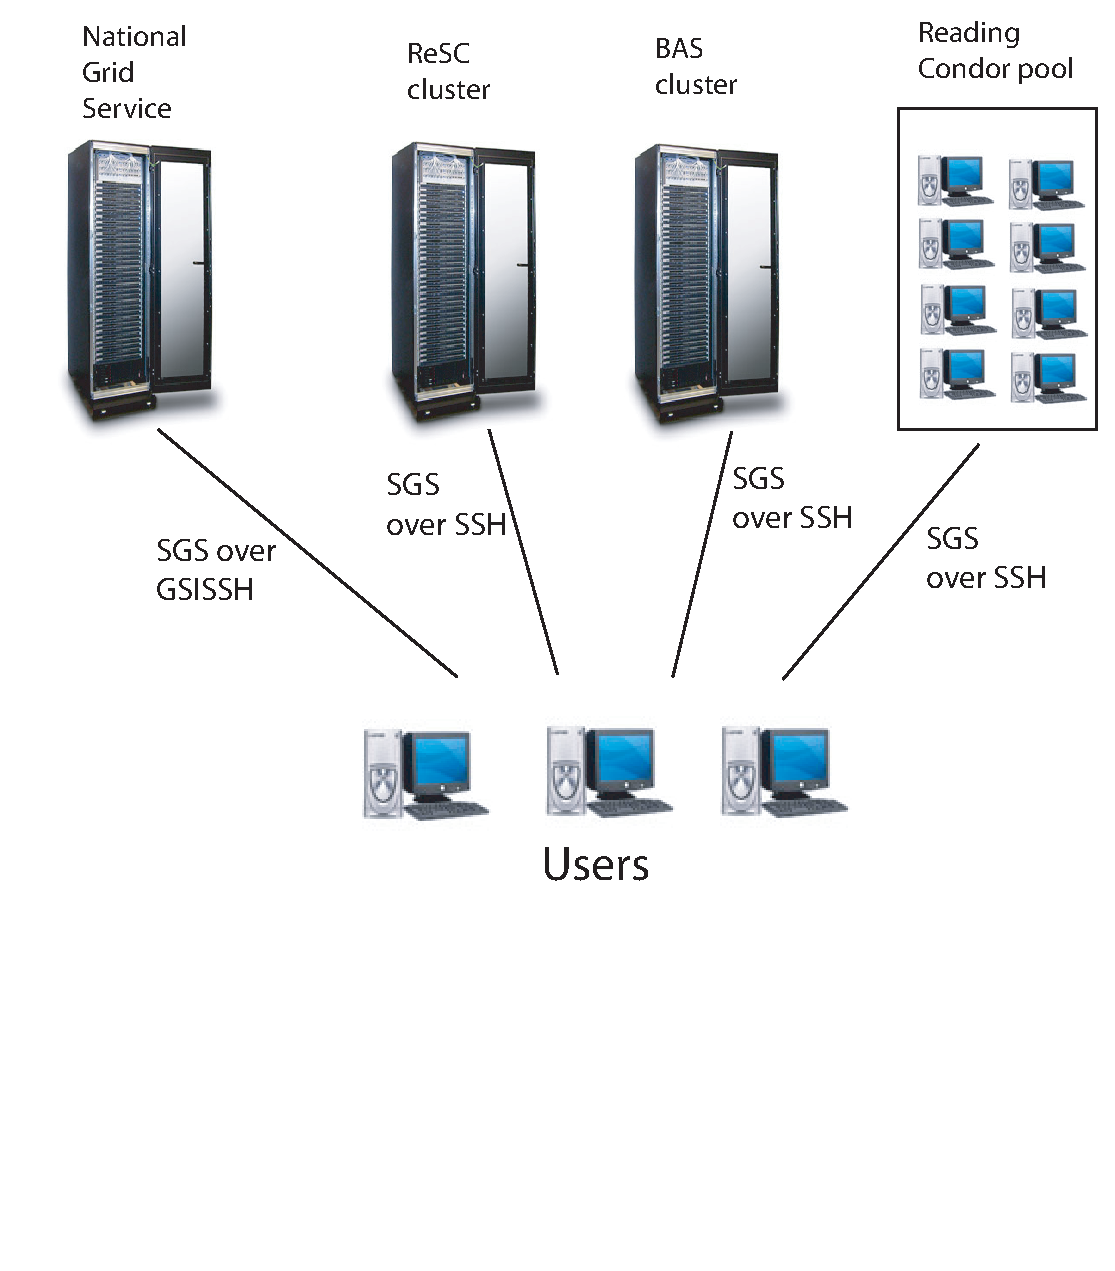
\includegraphics[height=8cm]{GCEP_architecture.eps}
\caption{Overview of the proposed architecture for the GCEP project, omitting the CCLRC cluster for clarity. The dedicated GCEP resources simply run SSH servers, as does the Reading Condor pool.  The National Grid Service resources are accessed through GSISSH.  The resources themselves run a variety of Distributed Resource Management systems including Condor and Sun Grid Engine.  The Styx Grid Services software is run over SSH and GSISSH to allow users to run Grid applications on these various resources just as easily as they would run local applications.  Files are shared amongst the resources using SSH and sshfs; the Storage Resource Broker is another option for this (section~\ref{sec:datamanagement}).} 
\label{fig:gcep}
\end{figure*}

There are two types of job that will be run in GCEP.  The first type is the running of the HadCM3 model itself to produce simulations of the evolution of the Earth's climate arising from various initial conditions.  HadCM3 is a complex model to configure and it only runs efficiently on certain clusters (e.g.\ it requires a large amount of memory per node).  Therefore, we expect that scientists will run the HadCM3 model ``manually'', by logging into the cluster in question (via SSH) and carefully configuring the program before running it.  This is an expert task that is not easily automated.

The second job type that will be run in GCEP is the analysis of the output from the HadCM3 model runs.  These data analysis jobs are typically much simpler to set up and can run on a wide variety of machines.  It is these data analysis jobs that are most suitable for automation using the Styx Grid Services system.  We propose that, when a scientist creates a useful data analysis tool (i.e.\ a program), he or she arranges for it to be installed on each of the GCEP resources as a Styx Grid Service.  All other scientists can then use this tool exactly as if they had it installed locally.  The SGS system would allow the tools to be run on a variety of resources (SGE clusters, Condor pools, individual machines) in a manner that is completely transparent to the scientists.

Although this does not use ``traditional'' Grid software, this is true Grid computing: it is distributed computing, performed transparently across multiple administrative domains.

\subsection{Using the National Grid Service}
When the GCEP scientists wish to use Globus resources such as the UK National Grid Service they will not be able to use SSH to access these resources directly.  There are two approaches to this:

\begin{enumerate}
\item Use GSISSH as a direct replacement for SSH: this uses the user's Grid certificate to authenticate with the server.  This requires the user to obtain and care for a certificate and create proxy certificates whenever he or she needs to run a job.
\item Create a ``gateway'' machine, which the user accesses through SSH as before. This gateway machine accesses the Globus resource on the user's behalf, creating the necessary proxy certificate automatically.  The user's certificate could be stored on this gateway machine (if it is sufficiently secure) or the certificate could be stored in a MyProxy server and retrieved automatically when the user runs a job.
\end{enumerate}

At the time of writing it is not clear which approach will be more appropriate for the project and further investigation will be required.

\subsection{Automatic resource selection}
A greater degree of transparency could be obtained by providing a system that automatically finds the best resource in the GCEP Grid on which a given job should run.  This might involve automatic selection of the ``fastest'' or ``least busy'' machine in the Grid to ensure that the scientists receive their results as quickly as possible.  Although an attractive idea in theory, this is very difficult to achieve in practice.  We envisage that the GCEP users will, initially at least, have to perform their own resource selection.  It may be possible to create a basic resource selector that queries the queue management system on each of the GCEP resources and makes a decision; however, this is unlikely to be optimal as it is extremely difficult to quantify the ``load'' on any given machine or to estimate the true length of a queue.

\subsection{Data management}\label{sec:datamanagement}
The GCEP project will produce several terabytes of data, which will be stored at the various partner institutions and which must be shared amongst the project scientists at all the institutions.  One option for handling this is to use the Storage Resource Broker (SRB).  This would create a single virtual data store that combines all the data stores at the partner locations.  Users would not have to know where each individual data file is stored: this is handled by the SRB system.  Additionally, the SRB system can store metadata about each file in the system, making it easier for scientists to find files in the entire virtual store.

An alternative approach, which would sacrifice some functionality but require less installation and configuration, would be simply to share the files via SSH.  Thanks to the widespread nature of SSH there are many tools for providing easy access to filesystems on an SSH server.  On Linux clients, remote filesystems that are exposed through SSH can be mounted on the client's machine through sshfs~\cite{sshfs}.  This has some significant advantages over SRB.  With sshfs, users would not have to copy entire data files to the location at which a particular data analysis program needs to run: the machine running the program can mount the remote disk via sshfs and operate upon the data file as if it were on a local disk.  This means that the data analysis program can extract just those portions of the data file that it needs, saving considerable file transfer time.  Sshfs is only available to Linux users (of which there are a large proportion in GCEP), although there is an equivalent, low-cost commercial equivalent (www.sftpdrive.com) available for Windows clients.  In the absence of sshfs, users can use SFTP (secure FTP) to move files from place to place.  An important limitation of an SSH-based distributed file system is that it lacks a dedicated metadata store.

\section{Discussion}
We have described how the ease of use of the Styx Grid Services system can be combined with the Secure Shell (SSH) to create Grid systems that are easy to build, use and administer.  No complex middleware is required and the barrier to uptake by users is very low: most of the tools involved are already familiar to a large proportion of users.  We have discussed how SGS-SSH can be applied to a multi-partner science project (GCEP), allowing compute and data resources to be shared transparently and securely with the minimum of administrative effort.  This will provide a reliable and easy-to-use Grid system to the GCEP scientists, allowing them to focus on the considerable science challenges rather than having to spend time learning new tools.

SGS-SSH does not provide every possible feature that might be desirable in a full-scale production Grid.  However, we argue that it provides enough features for most users and the simple nature of the system will, in many cases, more than make up for the missing features.  We hope that this will encourage more users and resource providers to create Grid systems to support collaborative science projects.

\section*{Acknowledgements}
This work was supported by the NERC Reading e-Science Centre grant and the NERC GCEP project grant.  The authors would like to thank Bruce Beckles for illuminating discussions on Grid security and the GCEP project partners for helpful suggestions and guidance.

\end{multicols}

\bibliographystyle{ametsoc}
\bibliography{refs}

\end{document}


